\section{Evaluation}\label{Evaluation}

In order to verify the feasibility of the proposed load balancer architecture, we evaluated it with the following criteria;
(1) Basic functionality and Portability:
We evaluated the load balancer functionality using physical servers in on-premise data center and compared performance level with existing iptables DNAT and nginx as a load balancer.
We also carried out the same performance measurement in GCP and AWS to show the containerized ipvs load balancer is runnable even in the cloud environment.
(2) Redundancy and Scalability:
We evaluated ECMP functionality by watching routing table updates on the router when the new load balancer is added or removed.
We also evaluated the performance level by changing the number of load balancers.

The following subsections explain the evaluation in detail.


%(3) Resource comsumption.
%We examined the basic performance of the our proposed load balancer container and the basic function of the ECMP redundancy using cluster of physical servers in on-premise data center.
%As for the performance, we measured throughput of the load balancer container and found that it was at least as good as existing software load balancer using Linux. 
%The ECMP redundancy is examined by . 
%We also demonstrate two different service with different number of load balancers can share the group of nodes.
%The portability of the load balancer is also evaluated using GCP and GCP.

\subsection{Basic functionality and portability}

\begin{figure}[t]
  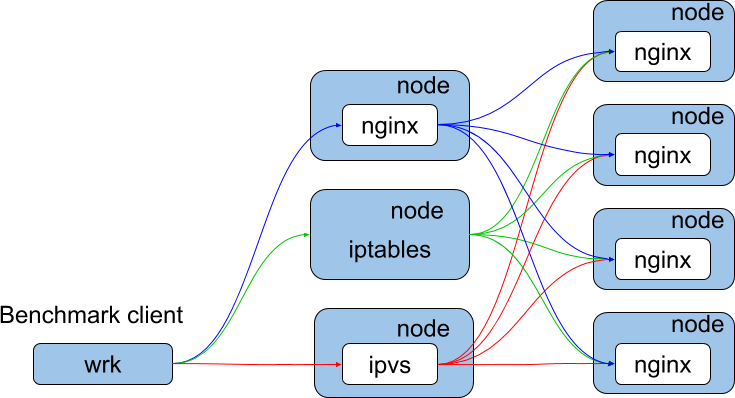
\includegraphics[width=0.9\columnwidth]{Figs/lb_single_schem}
  \caption{}
  \label{fig:lb_single_schem}
\end{figure}

\begin{figure}[t]

  \centering
\begin{Verbatim}[commandchars=\\\{\}]
───────────────────────────────────────────────────────
[Command line]
 wrk -c800 -t40 -d30s http://172.16.72.2:8888/
-c: concurrency, -t: # of thread, -d: duration

[Output example]
 Running 30s test @ http://10.254.0.10:81/
  40 threads and 800 connections
  Thread Stats   Avg      Stdev     Max   +/- Stdev
    Latency    15.82ms   41.45ms   1.90s    91.90%
    Req/Sec     4.14k   342.26     6.45k    69.24%
  4958000 requests in 30.10s, 1.14GB read
  Socket errors: connect 0, read 0, write 0, timeout 1
Requests/sec: 164717.63
Transfer/sec:     38.86MB
───────────────────────────────────────────────────────
\end{Verbatim}

    \caption{}
    \label{fig:bench_example}
\end{figure}

\begin{figure}[t]
\begin{Verbatim}[commandchars=\\\{\}]
───────────────────────────────────────────────────────
[Hardware Specification]
  CPU: Xeon E5-2450 2.10GHz x 8 (with Hyper Threading) 
  Memory: 32GB
  NIC: Broadcom BCM5720 Giga bit 
 (Node x 6, LB x 1, Client x 1)

[Node Software]
  OS: Debian 8.7, linux-3.16.0-4-amd64
  Kubernetes v1.10.6
  flannel v0.7.0
  etcd version: 3.0.15

[Container Software]
  Keepalived: v1.3.2 (12/03,2016)
  nginx : 1.15.4(web server) 
───────────────────────────────────────────────────────
\end{Verbatim}
    \caption{}
    \label{fig:hw_sw_spec}
\end{figure}


Throughput measurements were carried out in order to examine the basic functionality of the containerized ipvs load balancer.
Fig.~\ref{fig:benchmark-schem} shows the schematic diagram of the throughput measurement and summarizes experimental conditions.
We measured the performance of the load balancers using a benchmark program called wrk\cite{Glozer2016}.
Multiple nginx {\em pods} are deployed on multiple nodes as web servers in the Kubernetes cluster.
In each nginx {\em pod}, single nginx web server that returns the IP address of the {\em pod} is running.
We then set up the ipvs, iptables DNAT, and nginx load balancers on one of the nodes, and performed the throughput measurement.
The throughput is measured by sending out HTTP requests from the wrk towards a load balancer and by counting the number of responses the benchmark host received as shown in Fig.~\ref{fig:benchmark-schem}~(\subref{fig:lb_single_schem}).

Fig.~\ref{fig:benchmark-schem}~(\subref{fig:bench_example}) shows an example of the command-line for wrk and the corresponding output.
The command-line in Fig.~\ref{fig:benchmark-schem}~(\subref{fig:bench_example}) will generate 40 wrk program threads
and allow those threads to send out a total of 800 concurrent HTTP requests over the period of 30 seconds.
The output example shows information including per-thread statistics, error counts, throughput in [Request/sec] and data rate in [Transfer/sec]

Fig.~\ref{fig:benchmark-schem}~(\subref{fig:hw_sw_spec}) shows hardware and software configuration used in our experiments.
We used a total of eight servers; six servers for Nodes, one for the load balancer and one for the benchmark client, with all having the same hardware specifications.
The software versions used for Kubernetes, web server and load balancer {\em pods} are also summarized in the figure.

\begin{figure}[t]
  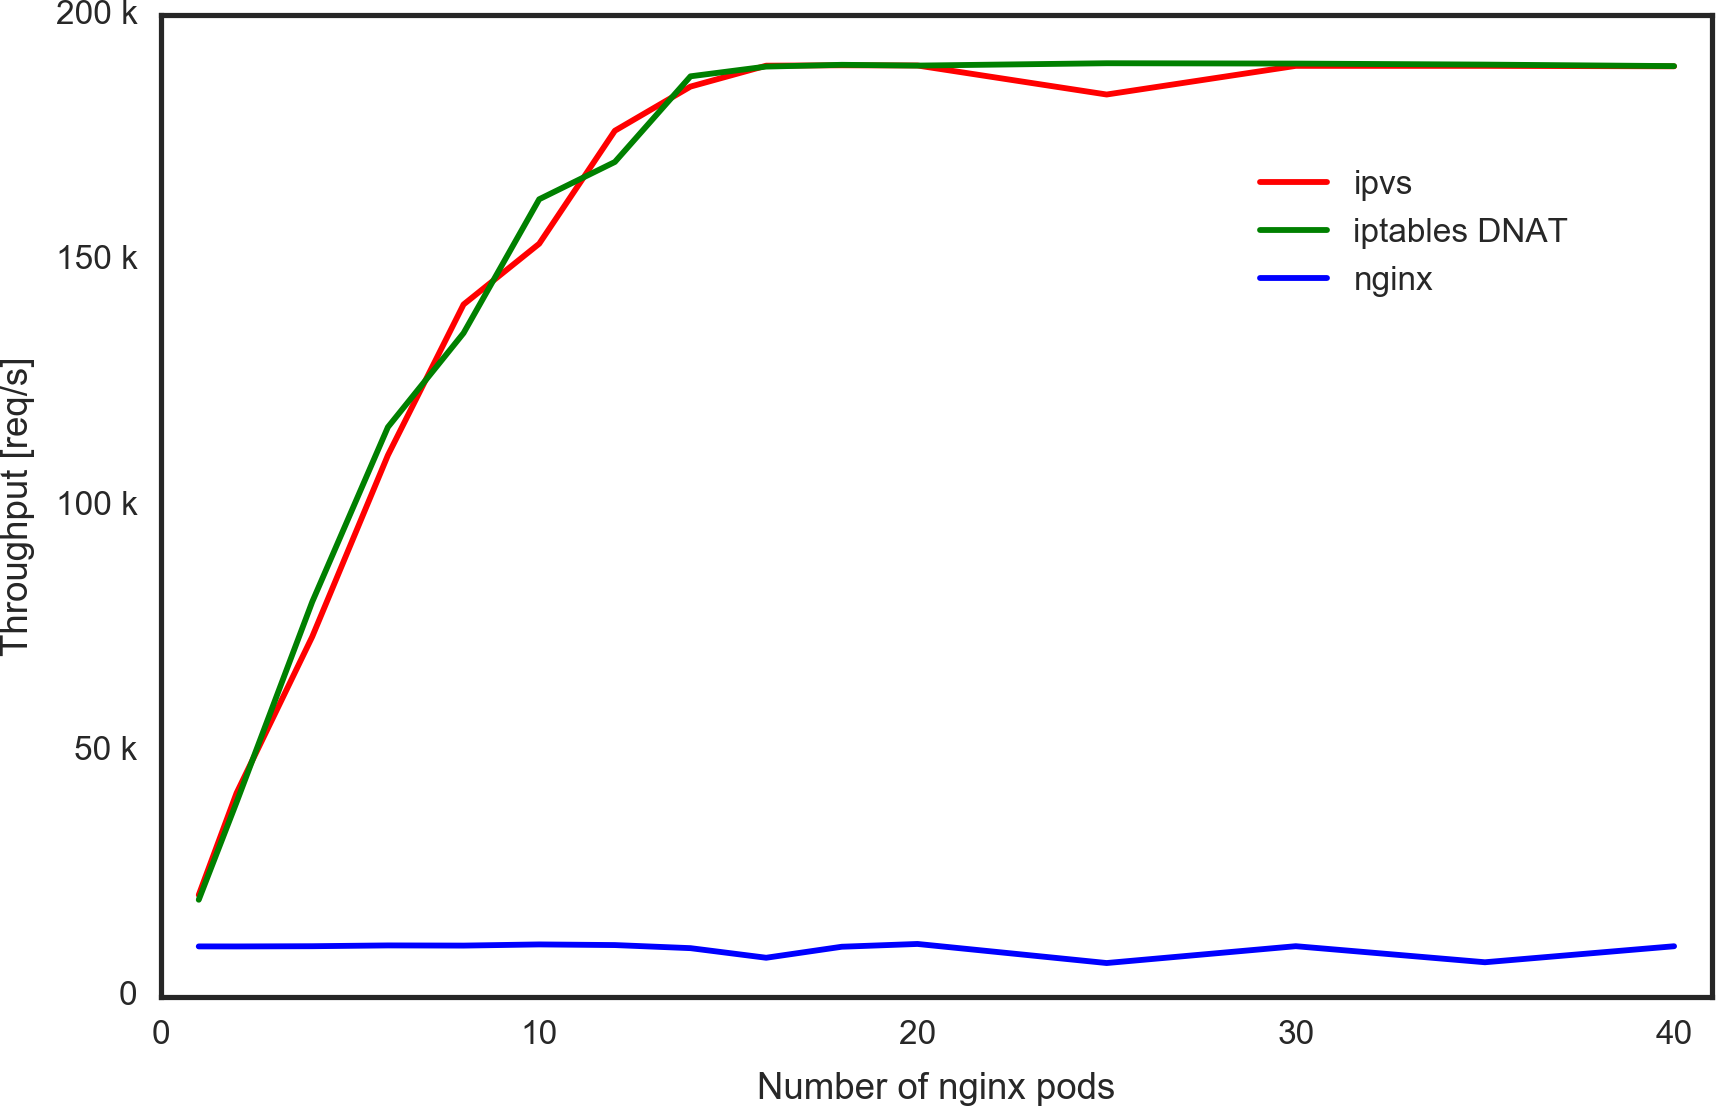
\includegraphics[width=0.9\columnwidth]{Figs/ipvs-iptables-nginx}
  \caption{Performance of the load balancer container.}
  \label{fig:ipvs-iptables-nginx}
\end{figure}


\begin{figure}[t]
    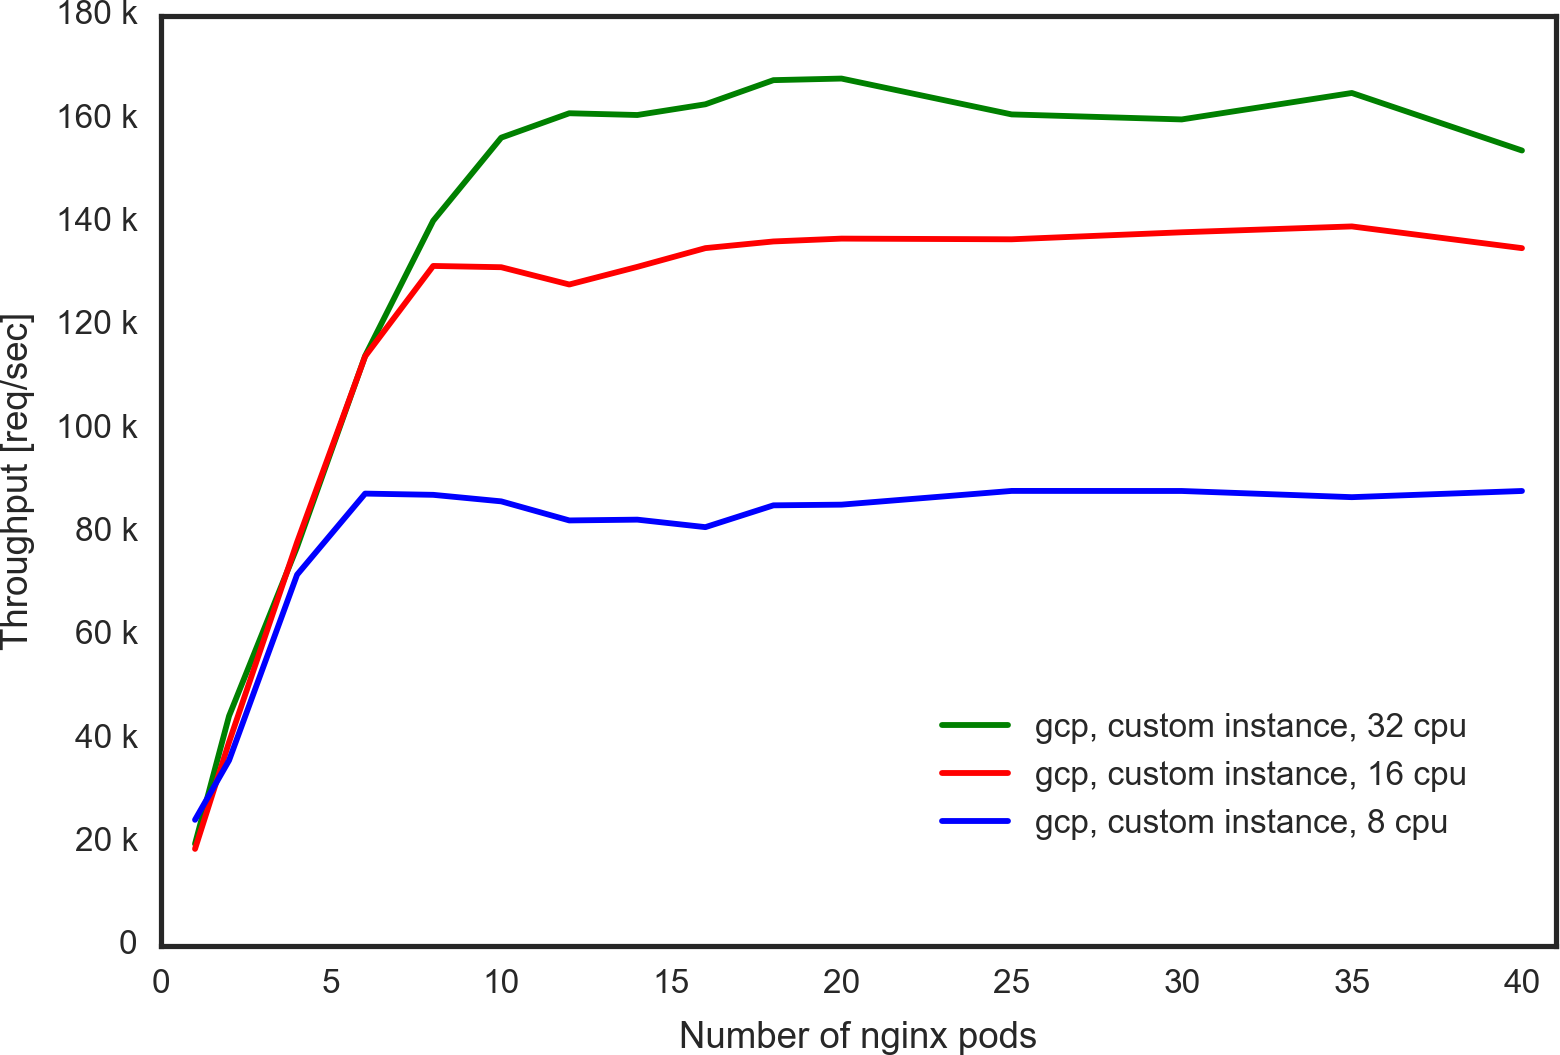
\includegraphics[width=0.9\columnwidth]{Figs/gcp_all_ieice}
    \caption{GCP}
    \label{fig:gcp_all_ieice}
\end{figure}

\begin{figure}[t]
    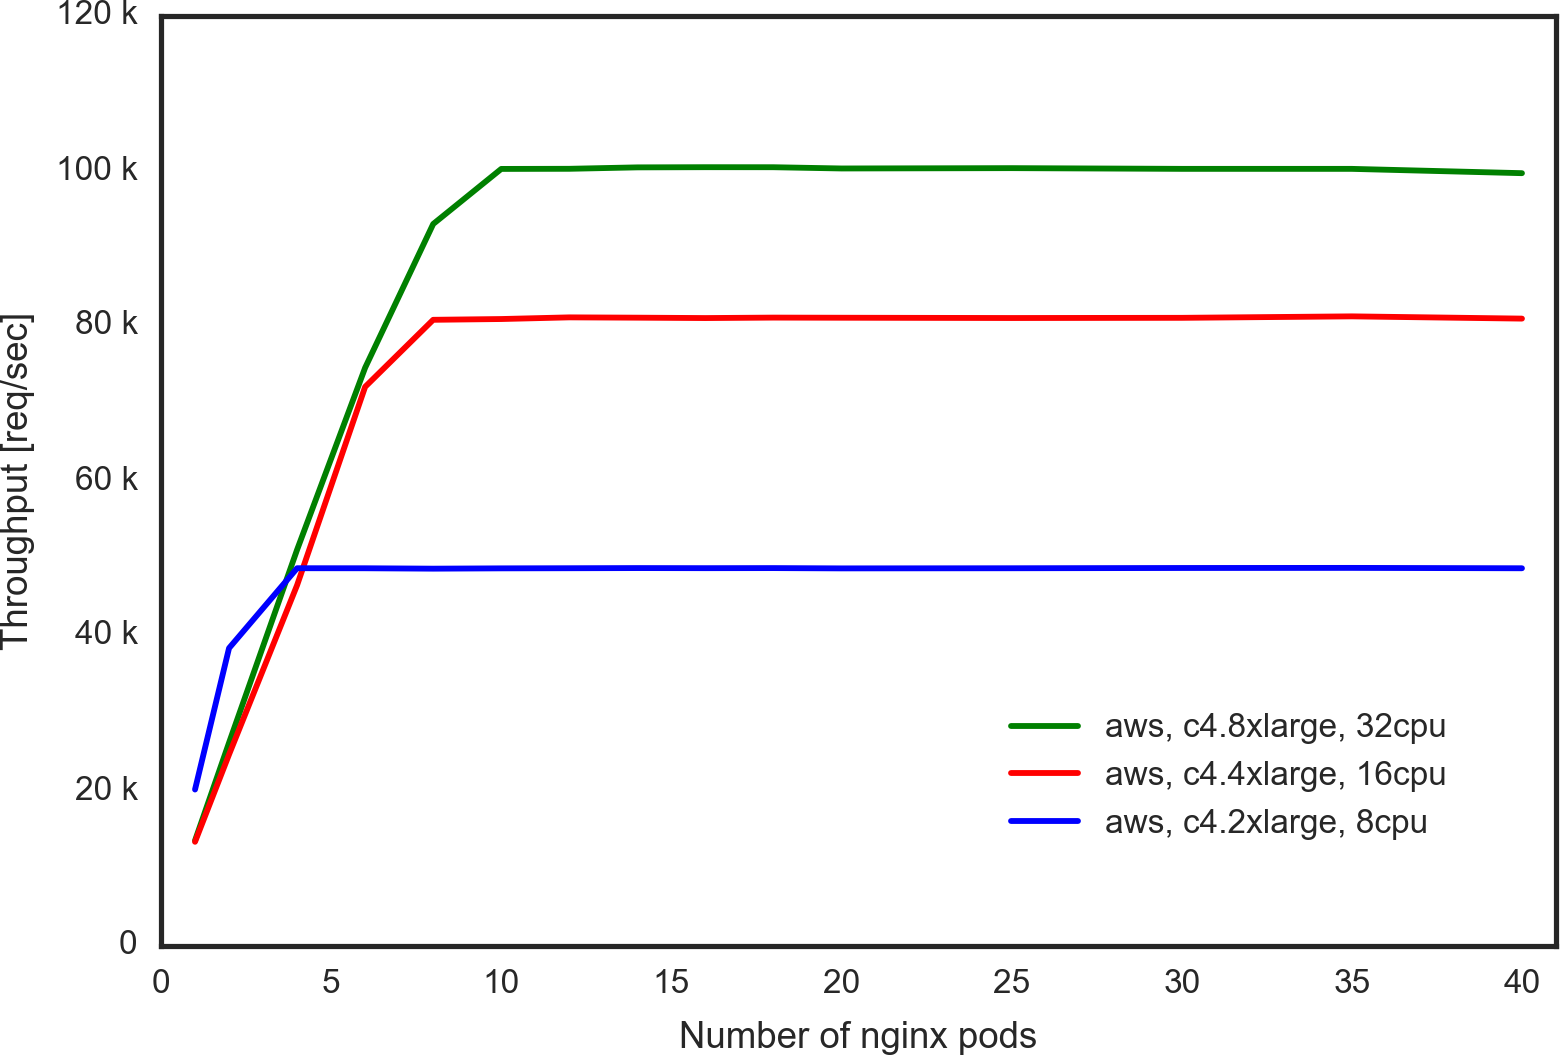
\includegraphics[width=0.9\columnwidth]{Figs/aws_c4_ieice}
    \caption{AWS with Node x 6, Client x 1, Load balancer x 1. Custom instance. }
    \label{fig:aws_c4_ieice}
\end{figure}

%\interfootnotelinepenalty=10000

Fig.~\ref{fig:ipvs_performance}~(\subref{fig:ipvs-iptables-nginx}) shows the throughput of the proposed ipvs container load balancer.
The performance of the nginx and the iptables DNAT as the load balancers are also presented for comparison.
As we increased the number of the nginx pods(web servers) from 1 to around 14, the throughput increased almost linearly and after which it saturated.
The increase indicates that the load balancer functions properly because it increased throughput by distributing HTTP requests to multiple of the web servers.
The saturated performance level indicates the maximum performance of the load balancer, which could be determined either by network bandwidth or CPU level of the load balancer or the benchmark client.
In this specific experiment, the performance level was limited by the 1 Gbps bandwidth of experimental network\cite{takahashi2018portable}, which is revealed by packet level analysis using tcpdump.\footnote{
On average the data size of each request was about 636 [byte/req] including TCP/IP headers, ethernet header, and interframe gaps.
Multiplying that with 190K [req/sec] and 8 [bit/byte] will result in 966.72 Mbps.
}
While nginx did not show any benefit as the load balancer, the performance of the ipvs load balancer container showed equivalent performance level as the un-containerized iptables DNAT.
This means that our proposed ipvs container load balancer is at least as good as the un-containerized iptables' load balancing in the 1 Gbps network.

Fig.~\ref{fig:ipvs_performance}~(\subref{fig:gcp_all_ieice}) and Fig.~\ref{fig:ipvs_performance}~(\subref{fig:aws_c4_ieice}) show the load balancer performance levels that are measured in GCP and AWS, respectively.
These are aimed to show that our proposed load balancer can be run in cloud environments and also functions properly.

Both results show similar characteristics as the experiment in an on-premise data center in Fig.~\ref{fig:ipvs_performance}~(\subref{fig:ipvs-iptables-nginx}), where throughput increased linearly to a certain saturation level that is determined by either network speed or machine specifications.
Since in the cases of cloud environments we can easily change the machine specifications, especially CPU counts, we measured throughput with several conditions of them.
From the first look of the results, since changing CPU counts changed the load balancer's throughput saturation levels, we thought VM's computation power limited the performance levels.
However, since there are cases in the cloud environment, where changing the VM types or CPU counts also changes the network bandwidth limit, a detailed analysis is further required in the future to clarify which factor limits the throughput in the cases of these cloud environments.
Still, we can say that the proposed ipvs load balancers can be run in GCP and AWS, and function properly until they reach the infrastructure limitations.


\subsection{Redundancy and Scalability}

The ECMP technique is expected to make the load balancers redundant and scalable since all the load balancer containers act as active.
We examined the behavior of the ECMP routing table updates, by changing the number of the load balancers.
After that, in order to explore the scalability, we also measured the throughput from a benchmark client with ECMP routes when multiple of the ipvs container load balancers are deployed.

\begin{figure}[b]
    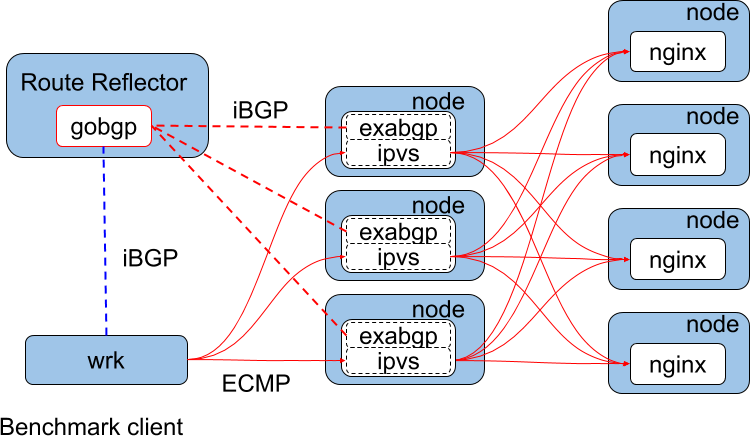
\includegraphics[width=0.9\columnwidth]{Figs/lb_ecmp_schem}
    \caption{}
    \label{fig:lb_ecmp_schem}
\end{figure}

\begin{figure}[t]
\begin{Verbatim}[commandchars=\\\{\}]
───────────────────────────────────────────────────────
[Hardware Specification]
  CPU: Xeon E5-2450 2.10GHz x 8 (with Hyper Threading) 
  Memory: 32GB
  NIC: Broadcom BCM5720 Giga bit 
 (Node x 6, Client x 1)

  CPU: Xeon E5-2450 2.10GHz x 8 (with Hyper Threading) 
  Memory: 32GB
  NIC: Intel X550
 (LB x 1)
  
[Node Software]
  OS: Debian 9.5, linux-4.16.8
  Kubernetes v1.5.2
  flannel v0.7.0
  etcd version: 3.0.15

[Container Software]
  Keepalived: v1.3.2 (12/03,2016)
  nginx : 1.11.1(load balancer), 1.13.0(web server) 
───────────────────────────────────────────────────────
\end{Verbatim}
    \caption{}
    \label{fig:ecmp-hw_sw_spec}
\end{figure}

Fig.~\ref{fig:ecmp-benchmark-schem} shows the schematic diagram of the experimental setup and also summarizes hardware and software specifications.
Notable differences from the previous throughput experiment in Fig.~\ref{fig:benchmark-schem} are as follows;
1) Each load balancer pods now consists of both an ipvs container and an exabgp container.
2) The routing table of the benchmark client is updated by BGP protocol through a route reflector.
3) The NIC of the benchmark client has been changed to 10 Gbps card since now we have multiple of ipvs container load balancers that are capable of filling up 1 Gbps bandwidth.
4) Some of the software have been updated to the most recent versions at the time of the experiment.

\begin{figure}[h]

\begin{subfigure}[t]{\columnwidth}
\centering
\begin{Verbatim}[commandchars=\\\{\}]
───────────────────────────────────────────────────────
10.1.1.0/24 via 10.0.0.106 \textbackslash 
                        dev eth0 proto zebra metric 20
───────────────────────────────────────────────────────
\end{Verbatim}
\caption{Routing table entry with single load balancer pod.}
\label{fig:single}
\end{subfigure}
\par\bigskip

\begin{subfigure}[t]{\columnwidth}
\centering
\begin{Verbatim}[commandchars=\\\{\}]
───────────────────────────────────────────────────────
10.1.1.0/24 proto zebra metric 20
        nexthop via 10.0.0.105  dev eth0 weight 1
        nexthop via 10.0.0.106  dev eth0 weight 1
        nexthop via 10.0.0.107  dev eth0 weight 1
───────────────────────────────────────────────────────
\end{Verbatim}
\caption{Routing table entry with three load balancer pods.}
\label{fig:three}
\end{subfigure}
\par\bigskip

\begin{subfigure}[t]{\columnwidth}
\centering
\begin{Verbatim}[commandchars=\\\{\}]
───────────────────────────────────────────────────────
10.1.1.0/24 pro to zebra metric 20
        nexthop via 10.0.0.107  dev eth0 weight 1
        nexthop via 10.0.0.105  dev eth0 weight 1
        nexthop via 10.0.0.106  dev eth0 weight 1
10.1.2.0/24 proto zebra metric 20
        nexthop via 10.0.0.107  dev eth0 weight 1
        nexthop via 10.0.0.106  dev eth0 weight 1
───────────────────────────────────────────────────────
\end{Verbatim}
\caption{Routing table entry with two services with two, three load balancer pods respectively.}
\label{fig:double_svc}
\end{subfigure}
\par\bigskip

\caption{ECMP routing tables.}
\label{fig:exabgp_routing_table}
\end{figure}

First, we examined ECMP functionality by watching the routing table on the benchmark client.
Fig.~\ref{fig:exabgp_routing_table}~(\subref{fig:single}) shows the routing table entry on the router when a single load balancer pod exists.
From this line, we can tell that packets toward 10.1.1.0/24 are forwarded to 10.0.0.106 where the load balancer pod is running.
It also shows that this routing rule is controlled by zebra.

When the number of the load balancer pods is increased to three, we can see the routing table entry in Fig.~\ref{fig:exabgp_routing_table}~(\subref{fig:three}).
We have three next hops towards 10.1.1.0/24 each of which being the node where the load balancer pods are running.
The weights of the three next-hops are all 1.
The update of the routing entry was almost instant as we increased the number of the load balancers.

Fig.~\ref{fig:exabgp_routing_table}~(\subref{fig:double_svc}) shows the case where we additionally started new service with two load balancer pods with service addresses in 10.1.2.0/24 range.
We could accommodate two different services with different IP addresses, one with three load balancers and the other with two load balancers on a group of nodes(10.0.0,105,10.0.0,106,10.0.0,107).
The update of the routing entry was almost instant as we started the load balancers for the second service.

We also carried out throughput measurement to show that our proposed architecture increases the throughput as we increase the number of the load balancers.
Fig.~\ref{fig:ecmp_scalability}~(\subref{fig:ecmp_lb_cubic_ieice}) shows the results of the measurements.
There are four solid lines in the figure, each corresponding the throughput result when there are one through four of the proposed load balancers.
%As can be seen in the figure, as we increased the number of the pod the thoroughput increased linearly to a certain level after which it saturated.
The saturated levels, i.e. performance levels depend on the number of the ipvs load balancer pods(lb x 1 being the case with one ipvs pods, and lb x2 being two of them and as such), which increases linearly as we increases the number of the load balancers.
The dotted line in the figure shows the throughput result when there were five load balancers.
It had almost the same performance level as the case when there were four load balancers, and did not scale further.
We suspect that this was because we used up CPU power of the benchmark client since the CPU idle was 0\% when there were more than four load balancers.
We expect that replacing the benchmark client with more powerful machines, or changing the experimental setup so that multiple benchmark clients can access the load balancers through an ECMP router, will improve the performance level further.

Fig.~\ref{fig:ecmp_scalability}~(\subref{fig:ecmp_response_ieice}) shows the throughput measurement results when we periodically changed the number of the load balancers. 
The red line in the figure shows the number of the ipvs load balancer pods, which we changed randomly every 60 seconds.
The blue line corresponds to the resulting throughput.
As we can see from the figure, the blue line nicely follows the shape of the red line.
This indicates that new load balancers are immediately utilized after they are created, and after removing some load balancers, the traffic to them is immediately directed to the existing load balancers.

Fig.~\ref{fig:ecmp_scalability}~(\subref{fig:ecmp_delay_histgram_ieice}) shows histogram of the ECMP update delay, where we measured the delays until the number of running ipvs pods is reflected in the routing table on the benchmark client, as we change the number of the ipvs pods randomly every 60 seconds for 20 hours.
As we can see from the figure, most of the delays are within 6 seconds, and the largest delay during the 20 hours experiment was 10 seconds.
We can conclude that ECMP routing update in our proposed architecture is quick enough.


  \begin{figure}[t]
    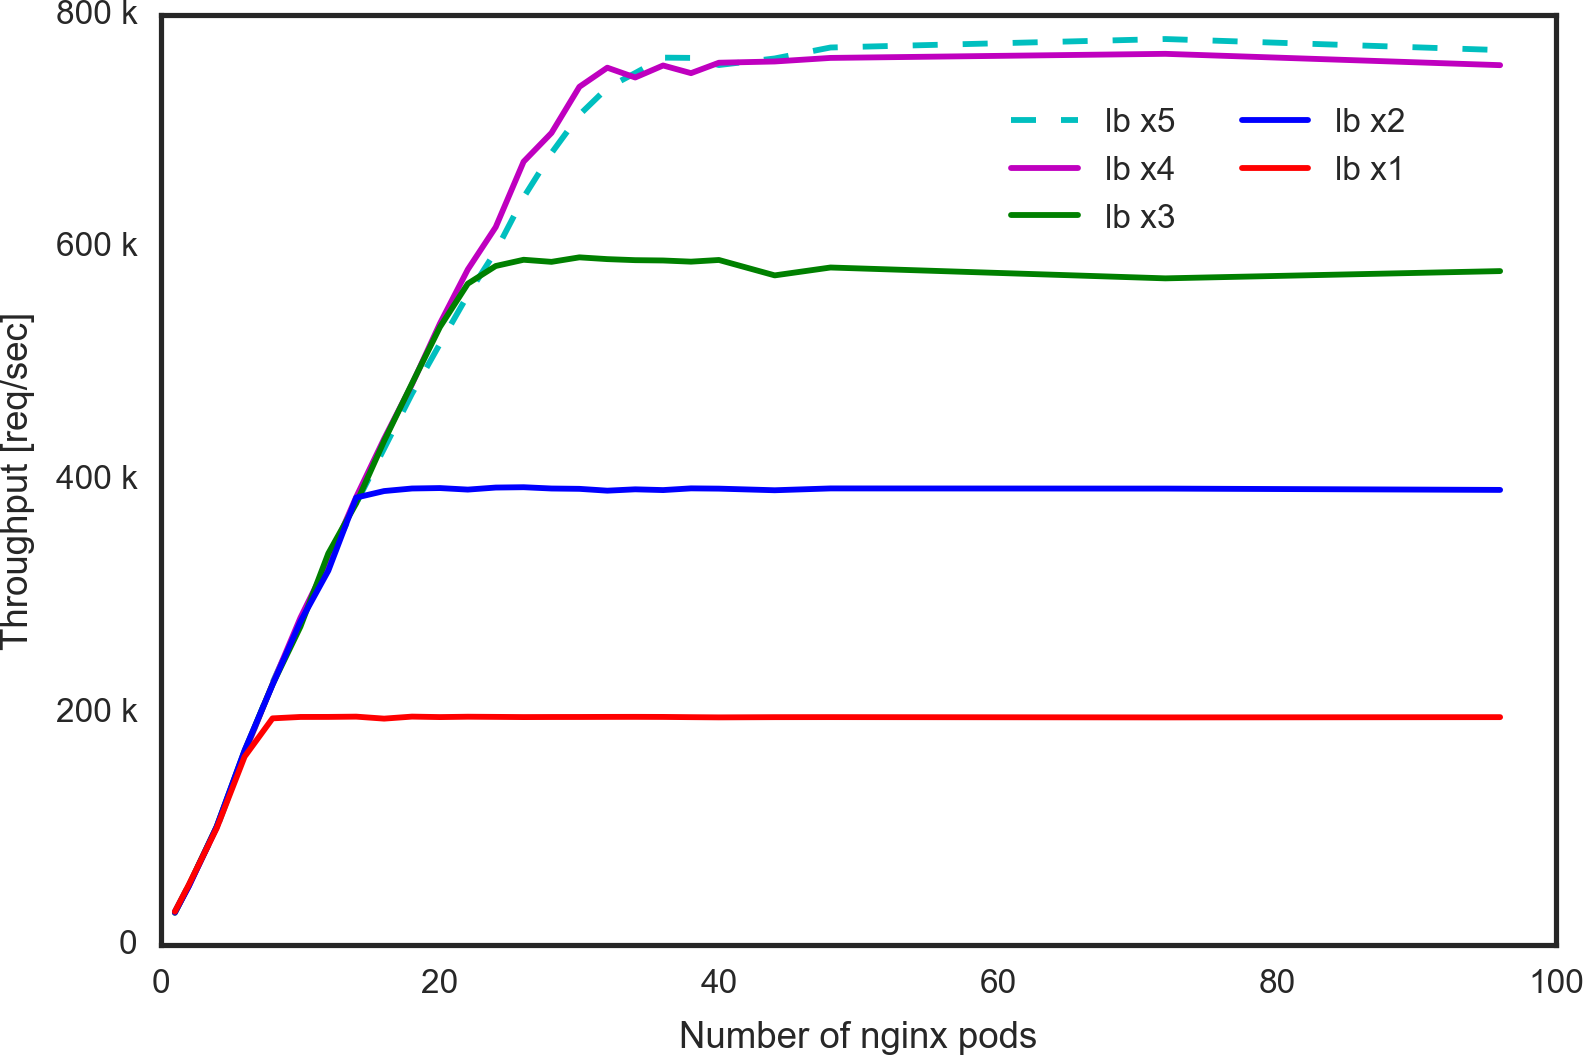
\includegraphics[width=0.9\columnwidth,left]{Figs/ecmp_lb_cubic_ieice}
    \caption{Caption 1}
    \label{fig:ecmp_lb_cubic_ieice}
  \end{figure}

  \begin{figure}[t]
    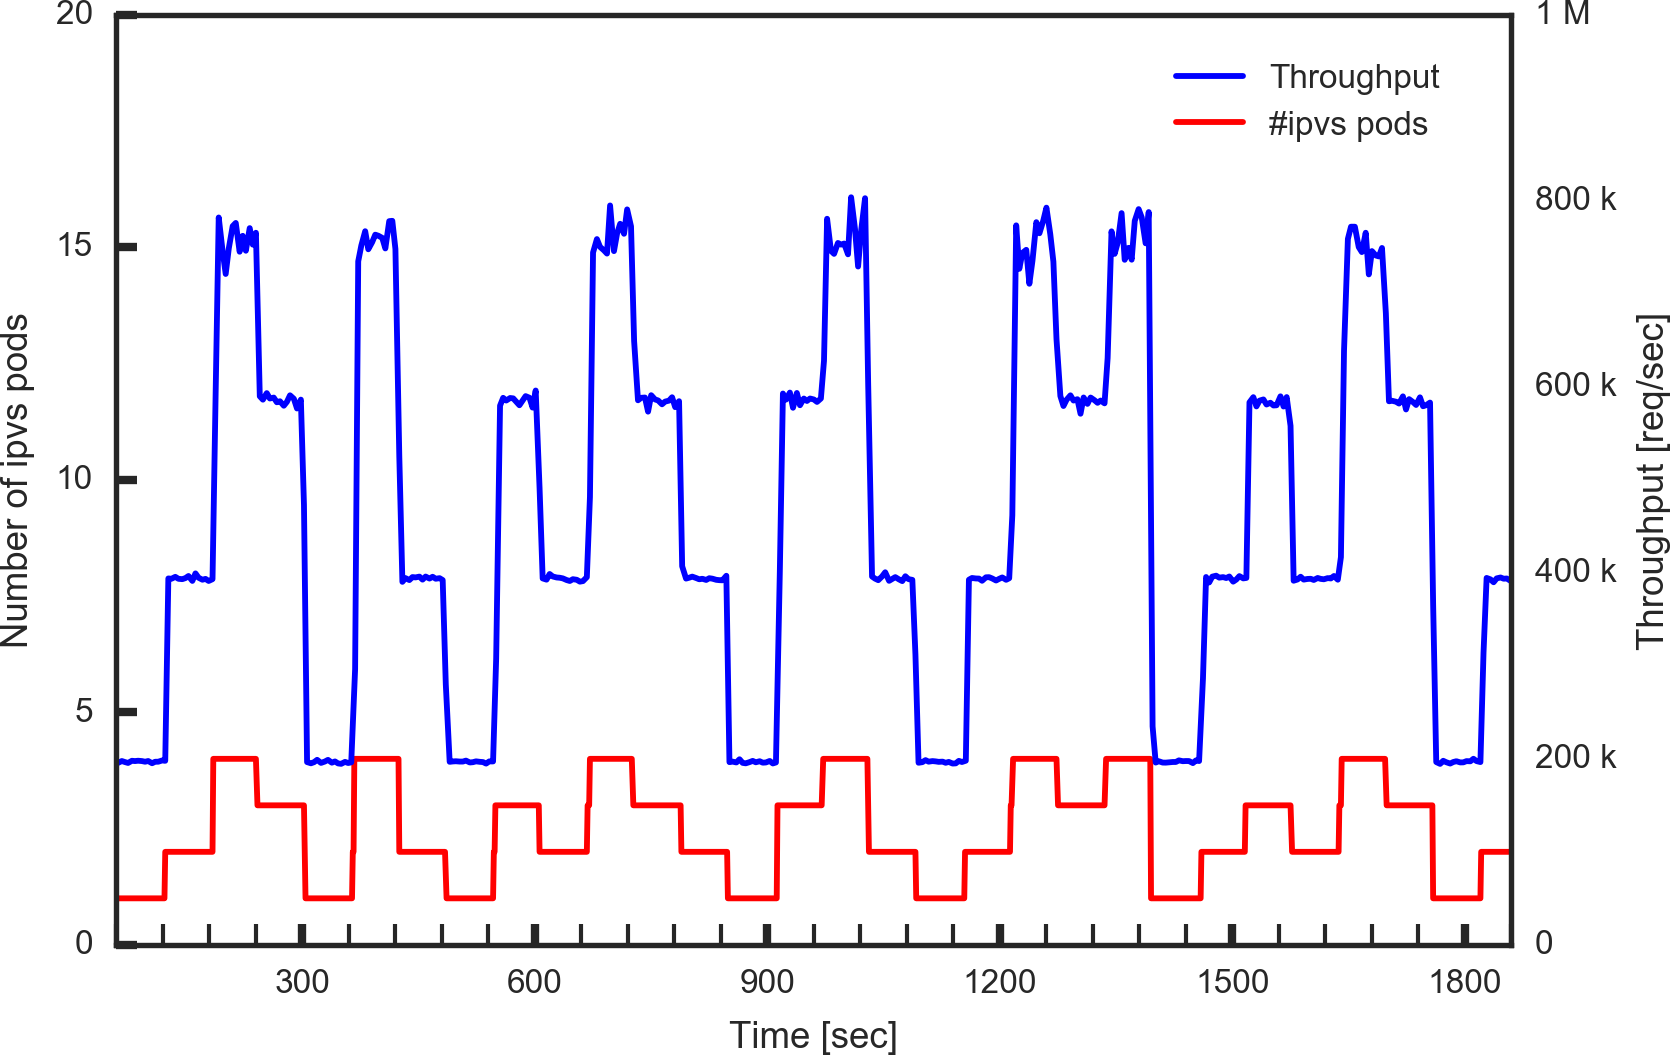
\includegraphics[width=0.98\columnwidth,left]{Figs/ecmp_response_ieice}
    \caption{Caption 2}
    \label{fig:ecmp_response_ieice}
  \end{figure}

  \begin{figure}[t]
    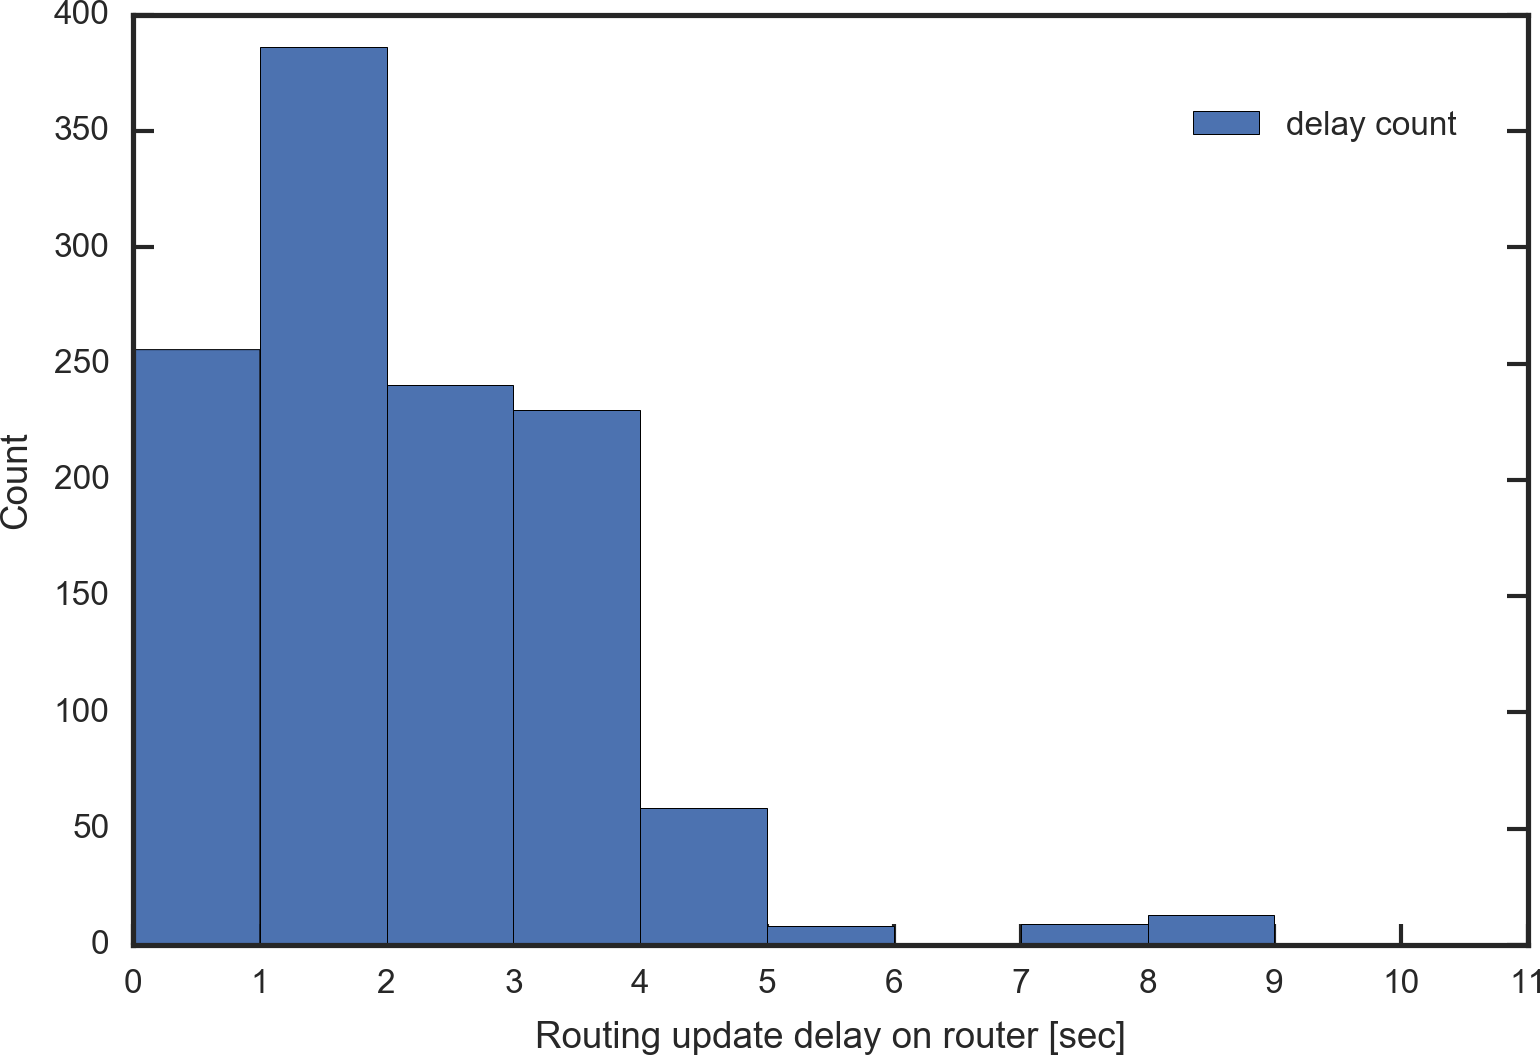
\includegraphics[width=0.9\columnwidth,left]{Figs/ecmp_delay_histgram_ieice}
    \caption{Caption 2}
    \label{fig:ecmp_delay_histgram_ieice}
  \end{figure}


\subsection{Resource Consumption}
